% =============================================================================
% HES-SO//Master Thesis Template
% =============================================================================

% Configuration
% -------------
% ==================
% Template settings
% ==================

\documentclass[a4paper,11pt,fleqn]{book}

% Language and encoding
% ---------------------
\usepackage[utf8]{inputenc}
\usepackage[T1]{fontenc}
\usepackage[english,french]{babel}


\selectlanguage{french}

% General tools
% -------------
\usepackage{etoolbox}

% Page style
% ----------
\usepackage[a4paper,top=25mm,bottom=25mm,inner=30mm,outer=20mm]{geometry}
\usepackage{fancyhdr}
\setlength{\headheight}{14pt}
\renewcommand{\sectionmark}[1]{\markright{\thesection\ #1}}
\pagestyle{fancy}
\fancyhf{}
\renewcommand{\headrulewidth}{0.4pt}
\renewcommand{\footrulewidth}{0pt}
\fancyhead[OR]{\bfseries \nouppercase{\rightmark}}
\fancyhead[EL]{\bfseries \nouppercase{\leftmark}}
\fancyfoot[EL,OR]{\thepage}
\fancypagestyle{plain}{
	\fancyhf{}
	\renewcommand{\headrulewidth}{0pt}
	\renewcommand{\footrulewidth}{0pt}
	\fancyfoot[EL,OR]{\thepage}}
\fancypagestyle{addpagenumbersforpdfimports}{
	\fancyhead{}
	\renewcommand{\headrulewidth}{0pt}
	\fancyfoot{}
	\fancyfoot[RO,LE]{\thepage}
}

% Use plain style for empty page when clearing
\makeatletter
\def\cleardoublepage{\clearpage\if@twoside \ifodd\c@page\else
	\hbox{}
	\thispagestyle{empty}
	\newpage
	\if@twocolumn\hbox{}\newpage\fi\fi\fi}
\makeatother \clearpage{\pagestyle{plain}\cleardoublepage}

% Fonts
% -----
\usepackage{tgheros}                       % Sans serif
\usepackage[bitstream-charter]{mathdesign} % Serif
\usepackage{sourcecodepro}                 % Monospace

% Math
% ----
\usepackage{amsmath}  % better math

% Floats and figures
% ------------------
\usepackage{float}                                  % floats
\usepackage[small,justification=centering]{caption} % captions
\usepackage{subcaption}

% Caption with source for figure
\newcommand*{\captionsource}[2]{%
	\caption[{#1}]{%
		#1%
		
		\textbf{Source:} #2%
	}%
}

% Tables
% ------
\usepackage{booktabs}
\usepackage{multirow}

% Bibliography
% -------------------
\usepackage[
backend=biber,
bibencoding=auto,
sorting=nty,
defernumbers=true
]{biblatex}
\addbibresource{03-tail/bibliography.bib}


% Colors & graphics
% -----------------
\usepackage[table]{xcolor}    % colors
\usepackage[pdftex]{graphicx} % graphics importing
\graphicspath{{img/}}
\definecolor{gray80}{gray}{0.80}

% Paragraphs
% ----------
\usepackage{csquotes}                    % paragraph indentation and spacing
\usepackage[defaultlines=3,all]{nowidow} % avoid widows and orphans
\usepackage{microtype}                   % typographic improvements
\usepackage{parskip}                     % No indent and auto-space between paragraphs


% Section and chapters headings
% -----------------------------
\usepackage{titlesec} % section titles formatting
\usepackage{sectsty}  % sectioning commands

% -- Sections --

% -- Chapters --
% Remove "Chapter N" and use a sans-serif font
\titleformat{\chapter}[block]
{\Huge}
{\thechapter\hspace{12pt}\textcolor{gray80}{|}\hspace{12pt}}
{0pt}
{\Huge\bfseries}

\titlespacing*{\chapter}
{0pt}
{-20pt}
{20pt}

% Use a sans-serif font
%\allsectionsfont{\sffamily\bfseries}


% Code and syntax highlighting
% ----------------------------
\usepackage{minted}   % code highlighting


% Page style
% -----------------


% References
% -----------
\usepackage{url}
\usepackage{hyperref}

% Misc
% ------
\usepackage{lipsum}    % filler text
\usepackage{lscape}    % easy landscape pages
\usepackage{pdflscape} % landscape pages for PDFs

% Glossary
% --------
\usepackage[xindy,toc]{glossaries}
% Terms
% -----
% format:  \newglossaryentry{<label>}{<settings>}
% example: \newglossaryentry{computer}
%{
%	name=computer,
%	description={is a programmable machine that receives input,
%		stores and manipulates data, and provides
%		output in a useful format}
%}
\newglossaryentry{nosql}
{
	name=NoSQL,
	description={Database not using the relational model and the \acrshort{sql} language}
}

% Acronyms
% --------
% format:  \newacronym{<label>}{<abbrv>}{<full>}
% example: \newacronym{lvm}{LVM}{Logical Volume Manager}
% plural:  \newacronym[longplural={Frames per Second}]{fpsLabel}{FPS}{Frame per Second}

% General
\newacronym{sql}{SQL}{Structured  Query Language}
\makeglossaries

\usepackage{listings}      % template settings
% ===========================================
% = Codestyles for minted syntax highlighting
% ===========================================


% How to use (replace 'java' with language name):
% - code blocks:
%     \begin{javacode}
%     CODE
%     \end{javacode}
% - files:
%     full: \javafile{PATH}
%     extract: \javafile[startline=x, endline=y]{PATH}

% Java
\newminted{java}{frame=single, framesep=6pt, breaklines=true, fontsize=\scriptsize}
\newmintedfile{java}{frame=single, framesep=6pt, breaklines=true, 
fontsize=\scriptsize}

% Scala
\newminted{scala}{frame=single, framesep=6pt, breaklines=true, fontsize=\scriptsize}
\newmintedfile{scala}{frame=single, framesep=6pt, breaklines=true, 
	fontsize=\scriptsize}

% Python
\newminted{python}{frame=single, framesep=6pt, breaklines=true, fontsize=\scriptsize}
\newmintedfile{python}{frame=single, framesep=6pt, breaklines=true, fontsize=\scriptsize}

% Plain text
\newminted{text}{frame=single, framesep=6pt, breaklines=true, breakanywhere, fontsize=\scriptsize}
\newmintedfile{text}{frame=single, framesep=6pt, breaklines=true, breakanywhere, fontsize=\scriptsize}       % code styles for minted
% ========================
% = TODO: Document
% ========================

%\cf{ch}{results}
\newcommand{\cf}[1]{chapitre~\ref{#1}-\nameref{#1}}  % your custom packages etc
% ========================
% = TODO: Document
% ========================

\newcommand{\Orientation}{MSE - Software Engineering}

\newcommand{\ThesisTitle}{Dockerisation d'environement pour Les projets de bioinformatique}

\newcommand{\Author}{Déruaz Vincent}

\newcommand{\Director}{Prof. Carlos Andrés Pena}
\newcommand{\DirectorResearchUnit}{CI4CB at HEIG-VD}

\newcommand{\ExternalExpert}{[Title] [FirstName] [LastName]\\Company/Lab}

\newcommand{\Place}{Lausanne}

         % thesis + school info

\begin{document}

% ----------------------------------------------------------------------------
% Frontmatter
% ----------------------------------------------------------------------------
\frontmatter

% ==========================================================================
% = HES-SO Master thesis title page (modeled after Word template, 2016-2017)
% ==========================================================================

\begin{titlepage}
	\begin{flushright}
		\begin{minipage}{0.5\textwidth}
			\begin{flushleft}
				
\includegraphics[width=0.9\textwidth]{mse_logo}
			\end{flushleft}
		\end{minipage}%
		\begin{minipage}{0.5\textwidth}
			\begin{flushright}
				
\includegraphics[width=0.6\textwidth]{hesso_logo}
			\end{flushright}
		\end{minipage}
		\begin{flushleft}
			\footnotesize
			Master of Science HES-SO in Engineering \\
			Av. de Provence 6 \\
			CH-1007 Lausanne
		\end{flushleft}
		~\\[0.5cm]
		
		{
		\Huge Master of Science HES-SO in Engineering\\[0.5cm]
		}
		
		{
		\LARGE Orientation: Information and Communication Technologies (ICT)\\[0.5cm]
		~\\[1cm]
		}
		% Title
		{
			\Huge
			\ThesisTitle \\[1.5cm]
		}
		{
			\large
			Autheur:\\[-0.3cm]
			\Huge \Author \\[0.8cm]
		}
		{
			\large
			Sous la direction de: \\
			\Director \\
			\DirectorResearchUnit \\[0.5cm]
		}
		\vfill
		
		% Bottom of the page
		{\large \Place, HES-SO//Master, \today}
		
	\end{flushright}
\end{titlepage}


 % don't modify, it follows the MSE mandatory format
\cleardoublepage
\thispagestyle{empty}


\vspace*{3cm}

\begin{raggedleft}
    	Sometimes a scream is better than a thesis.\\
     --- Manfred Eigen\\
\end{raggedleft}

\vspace{4cm}

\begin{center}
    To my parents\dots
\end{center}



\setcounter{page}{0} % start numbering here
\chapter*{Acknowledgements}
\markboth{Acknowledgements}{Acknowledgements}
\addcontentsline{toc}{chapter}{Acknowledgements}

Cette thèse as àtà réalisé dans le cadre du projet Inphinity à l'HEIG-VD.

Elle fait suite à la thèse de master [TODO: TITLE] réalisée par [TODO: prenom+nom DIOGO].

%TODO: explication these diogo (une courte phrase + details ci-après CH2)
 

%\begingroup
%\let\cleardoublepage\clearpage


% English abstract
\cleardoublepage
\chapter*{Abstract}
%\markboth{Abstract}{Abstract}
\addcontentsline{toc}{chapter}{Abstract (English/Français)} % adds an entry to the table of contents
% put your text here
\lipsum[1-2]
\vskip0.5cm
Key words: 
%put your text here


% French abstract
\begin{otherlanguage}{french}
\cleardoublepage
\chapter*{Résumé}
%\markboth{Résumé}{Résumé}
% put your text here
\lipsum[1-2]
\vskip0.5cm
Mots clés: 
%put your text here
\end{otherlanguage}


%\endgroup			
%\vfill


% Table of contents
\tableofcontents
\cleardoublepage

% List of figures
\phantomsection
\addcontentsline{toc}{chapter}{List of figures} % adds an entry to the table of contents
\listoffigures
\cleardoublepage

% List of tables
\phantomsection
\addcontentsline{toc}{chapter}{List of tables} % adds an entry to the table of contents
\listoftables

% TODO: List of listings

% Restore space between paragraphs (was 0 for tables)
\setlength{\parskip}{1em}

% ----------------------------------------------------------------------------
% Mainmatter
% ----------------------------------------------------------------------------
\mainmatter

% Put your chapters here...
\chapter{Introduction}
\label{ch:introduction}

Ce travail à été réalisé la la suite d'une autre thèse de master dont l'interet était de prouvé la pertinence d'une méthode d'analyse par \emph{machine learning}. En effet, il s'agit d'une méthode permettant [TODO: completer].

Dans la présente thèse il est question de mettre en place plusieurs aspect permettant l'anrichissement du processus d'analyse de la thèse \emph{[TODO: these name of diogo]}. 

Notamment, l'utilisation de python 3 pour remplacer l'utilisation de python2, moins efficace. %TODO: proof

De plus, ont souhait être capable d'automatiser le lancement de "l'application" et par la même occasion rendre le déploiement facile et unifier quelque soit la machine cible, pour autant qu'elle utilise le système d'exploitation Linux.

Troisièmement, on souhaite pouvoir lancer l'analyse pour différentes configuration, créées à l'avance.

Un objectif important, était de remplacer l'utilisation à une API en ligne par une utilisation local cf.\cf{ch:setup}.

Afin de réaliser ces objectif une première phase du travail à consisté à realiser des états de l'art pour les différents domaines utilisé (cf.\cf{ch:state_art}). %TODO: link to chapter 3


%%%%%%%%%%%%%%%%%%%%%%%%
%TODO: Information concernant la volonté de réaliser un Docker for Bio-Informatique
%%%%%%%%%%%%%%%%%%%%%%%%
%\chapter{Approche}
\label{ch:approche}


\chapter{Etats de l'art}
\label{ch:state_art}

\section{Introduction}
Dans ce chapitre, nous aborderons les différentes pistes envisagées afin de remplir les objectifs fixés dans cette thèse, comme listés dans l'introduction (\cf{ch:introduction}).

Avant toutes choses, il a fallu se mettre au niveau et comprendre la thèse \thLeite.

\section{Automatisation}
En terme d'automatisation, une pratique bien courante chez les développeurs s'agit d'utiliser des scripts bash afin de pouvoir exécuter un certain nombre de commandes et de codes successivement. Bien que cette méthode présente l'avantage d'être simple, il suffit d'une console UNIX et d'un éditeur de texte, elle présente un défaut majeur. En effet, le développeur du script contrôle quelle commande et code sont exécutés et peut également définir des paramètres pour ceux-ci, mais il ne peut pas contrôler l'environnement d'exécution.

Une façon de faire, en plein essor depuis quelque temps, est l'utilisation de la plateforme Docker \cite{1}. Il s'agit d'un logiciel de containerisation. C'est-à-dire la création de briques d'applications, qui mises ensemble permettent de réaliser une application globale. De plus, le développement d'une telle solution permet un partage facilité grâce à un déploiement facilité et autonome. Pour davantage d'explications sur le sujet je vous renvoie au  \cf{ch:docker}.

Vous l'aurez bien compris, le choix qui a été fait est celui de l'utilisation de Docker.

\section{Configuration}

En ce qui concerne la recherche d'une méthode afin de réaliser facilement des fichiers de configurations précréées, beaucoup de solutions existent. Ces différentes méthodes sont plus ou moins flexibles aux modifications.

Les fichiers de configurations dont il est question ici sont spécifiques à la partie python du code qui sera exécuté par notre application \cf{ch:app}. En effet, l'on souhaite entre autres être capable de donner des fichiers de configuration en entrée et d'obtenir pour chacun un résultat en sortie.

Nous citerons ici uniquement la solution retenue, car les autres solutions trouvées sont soit trop incompatibles soit presque identiques à la solution retenue.

Nous utilisons le module python \emph{Configparser} \cite{13}, qui permet de lire et parser des fichiers à l'extension .ini de manière simple. De plus, la structure d'un fichier .ini est très simple et ne laisse donc que très peu de place aux erreurs de format.
 
 
\section{Hmmer}
Dans la thèse \thLeite les séquences protéiniques sont recherchées dans la base de données de profile-HMM à l'aide d'une \gls{api} en ligne. Cette \gls{api} est disponible depuis le site \emph{https://www.ebi.ac.uk/Tools/hmmer/} \cite{19}. 

Comme dit précédemment, un des objectifs de ce travail est de se passer de l'utilisation de cette \gls{api} car son accès n'est pas toujours disponible ou stable.

Une recherche rapide a permis de se rendre compte que l'application utilisée derrière cette \gls{api} est disponible au téléchargement et peut donc être utilisée de manière locale. Pour davantage d'information \cf{ch:app}, sous-chapitre Hmmer.


\section{Parallélisation}

La version existante du code se trouvant dans la thèse \thLeite est une version sous forme de script, proof-of-concept, en python2 et non \emph{multiprocessed}. Afin de garantir une utilisation optimale des ressources de la machine hôte, sur laquelle le code est exécuté, nous souhaitons rendre le code parallèle là où il est possible de le faire.

Plusieurs solutions sont possibles, encore une fois les solutions les plus compliquées ne sont pas toujours les plus efficaces. De plus une méthode trop complexe pourrait réduire la bonne transmission du code à d'autres développeurs.

La partie principale que l'on souhaite paralléliser est l'utilisation de la fonction de scanne de HMMMER, étant donné qu'un très grand nombre de séquences protéiniques doivent être analysées.

\newpage
\subsection{Simple}
\subsubsection{Docker}
Docker, mis à part de rendre le déploiement et l'exécution d'application automatisée, permet également de lancer plusieurs conteneurs simultanément, \cf{ch:docker}. Un conteneur englobe un système de fichier complet possédant tout ce qui est nécessaire à remplir sa fonction. 

\subsubsection{Python}
En python on retrouve deux principales méthodes permettant de réaliser de code parallèle. En effet, on peut utiliser le \emph{multiprocessing} ou le \emph{multithreading}.

Notre but est de réaliser et d'optimiser un code \gls{cpu} dépendant, c'est-à-dire coeurs dépendants. Lors de l'utilisation du langage python il faut savoir qu'avec des codes \gls{cpu} dépendants, python limite les possibilités de parallélisme à cause de la \gls{gli}. La \gls{gli} est nécessaire en python, car python n'est pas \emph{tread safe}. En effet, il y a, en python, un verrou global lorsque l'on essaye d'accéder à un objet depuis un thread.

À cause de se verrou les codes \gls{cpu} dépendants ne gagneront pas en performance lorsqu'ils sont parallélisés à l'aide de \emph{multithreading}, mais uniquement avec le \emph{multiprocessing}.

\subsection{Avancée}
\subsubsection{Docker Swarm}
Une autre méthode utilisant une librairie avancée de Docker, consiste à utiliser Docker Swarm \cite{9}. Docker Swarm apporte à Docker une gestion native du \emph{clustering}, afin de transformer un groupe de \emph{Docker engines} en un unique et virtuel \emph{Docker engine}. Grâce à cela, il est possible d'exécuter une application sur une architecture partagée sur plusieurs systèmes physiquement indépendants. 

\subsubsection{Spark}
Spark \cite{6},\cite{7} est un framework \emph{open source} de calcul distribué. Il permet d'effectuer des analyses complexes sur un grand nombre de données.

Il est également un ensemble d'outils pour le traitement de grandes sources de données, notamment grâce à des fonctions \emph{MapReduce}.
	
\section{Optimisations}
Le code repris de la thèse \thLeite est un code séquentiel, sous forme de script nécessitant des inputs utilisateurs à chaque étape. De plus, ce code est écrit en python dans sa version 2.

Grâce au travail du Dr. Brett Cannon, \href{https://speakerdeck.com/pyconslides/python-3-dot-3-trust-me-its-better-than-python-2-dot-7-by-dr-brett-cannon}{voir ici}, on se rend compte que python 3.3 pourrait optimiser les performances de notre application. On peut lire  \href{https://mail.python.org/pipermail/python-dev/2012-October/121923.html}{ici} que même l'appel des fonctions est en moyenne 1.20 fois plus rapide. De plus, les \emph{threadded count} sont également plus rapides.

Une autre possibilité est d'utiliser \emph{Cython} \cite{11}. Cython est un compilateur/langage de python permettant d'utiliser des appeles au langage C et de compiler un code python en exécutable C. Il faut savoir qu'un exécutable C est généralement plus rapide que l'exécution de l'interpréteur Python. 

On trouve le tableau suivant dans la documentation de Cython, qui permet de nous rendre compte des différences.

\begin{figure}[H] 
\centering 
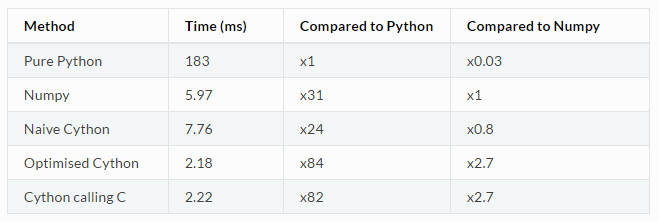
\includegraphics[width=1\columnwidth]{img/table_cython} 
\caption[Tableau performences Cython]{Tableau de comparaison de Cython - \url{http://notes-on-cython.readthedocs.io/en/latest/std_dev.html/}).}
\label{fig:galleria} 
\end{figure}

\section{Conclusion}
Après des tests sur ces différentes technologies et méthodes et quelques discussions ici et là, l'idée ayant été arrêtée est d'utiliser \emph{Docker} et \emph{Docker Compose} comme contexte applicatif et de transformer les scripts en une application orientée objet en python 3.3 gérant les fichiers de configurations avec la librairie \emph{Configparser}. Pour ce qui est du parallélisme, il sera réalisé en utilisant la librairie \emph{Multiprocess}.

















\chapter{Bases de Docker}
\label{ch:docker}

\section{Introduction}
Dans ce chapitre nous allons parler du fonctionnement de \emph{Docker} et \emph{Docker Compose}. Ce chapitre est réalisé sous le ton d'un cours d'introduction à Docker, afin de pouvoir transmettre les connaissances de base a l'utilisation et à la modification du travail réalisé lors de cette thèse. Cela passera entre autres par certains exemples et codes qui seront fournis en annexe notamment.

Docker permet l'exécution de code dans un conteneur indépendant de vote système hôte. 

\subsection{Utilisations}
\subsection{Compatibilité inter-OS}
Docker permet d'éviter les problèmes liés aux différences entre les environnements d'exécution. En effet, lorsque l'on exécute un code avec Docker ont contrôlé exactement l'état et le type d'environnement d'exécution. Cela rend donc possible l'exécution d'un code sous différent \gls{os} hôte (OSX, Linux, Windows).

Mais pourquoi ne pas utiliser une simple machine virtuelle ? Une première différence entre une machine virtuelle et Docker est le fait que Docker n'encapsule pas tout un \gls{os}, ceci permet une exécution beaucoup plus rapide, et c'est bien se que l'on cherche dans ce travail.

\begin{figure}[H] 
\centering 
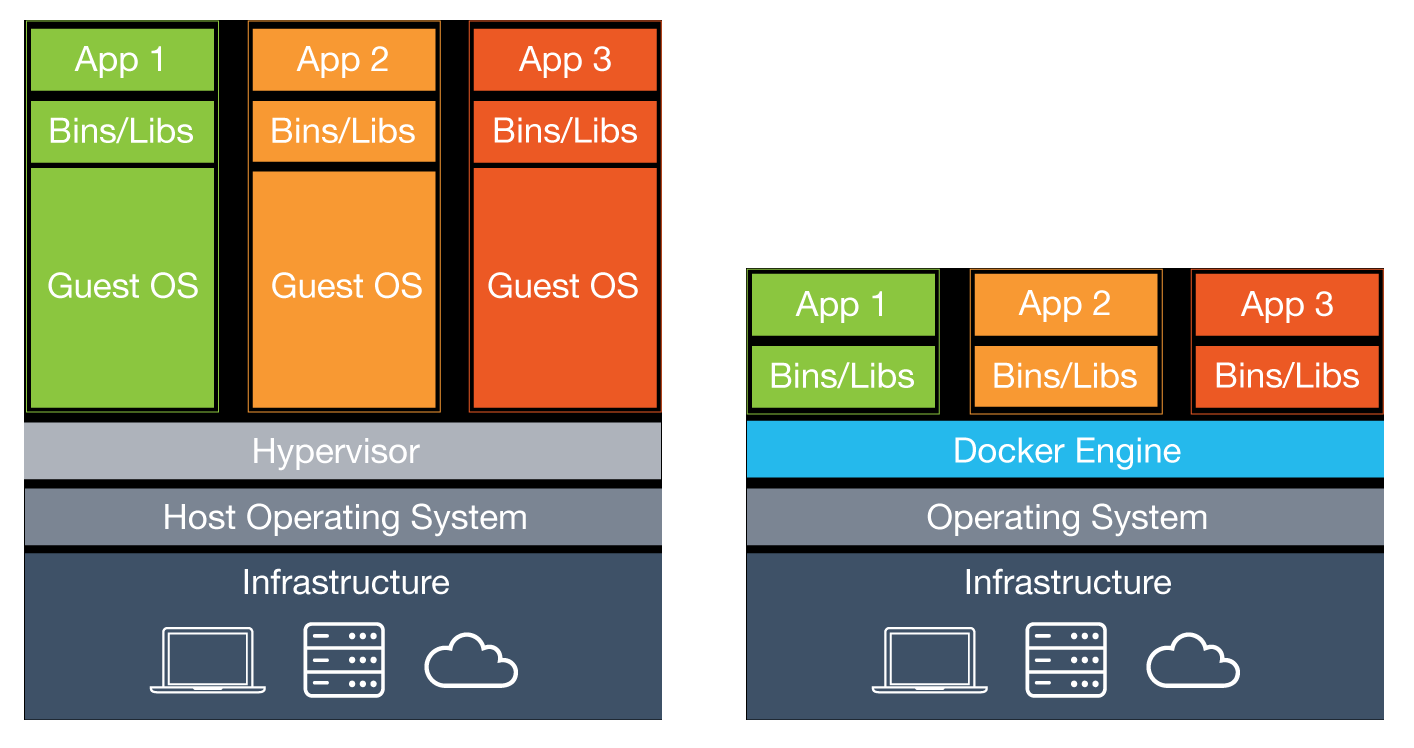
\includegraphics[width=1\columnwidth]{img/vm-vs-docker-container} 
\caption[vm vs Docker]{Virtual machine vs Docker}
\label{fig:vs} 
\end{figure}

\subsection{Miracle or illusion}
Je tiens ici à faire une mise en garde vis-à-vis de l'utilisation de Docker. Dans sont utilisation Docker est, à mon sens, une solution assez miraculeuse, notamment par le fait que l'on peu partage une application sans se poser de question sur l'hôte cible. Mais attention Docker n'est pas aussi miraculeux que cela dans le développement d'une solution applicative. En effet, il peut parfois êtres compliquer d'arriver du premier coup à réaliser se que l'on souhaite.

Docker n'est donc pas une solution miracle, mais présente beaucoup d'avantages en termes d'exécution standardisée, de partage de code et de déploiement.

\section{Pré-requis}
\subsection{Connaissance}
Il est nécessaire d'êtres à l’aise avec l'\gls{os} Linux et l'utilisation de commande UNIX. En effet, la plupart du temps les conteneurs utiliseront un système Linux. Pour plus d'information cf. ci-après.


\subsection{Installations}
\lstset{language=bash}
\lstset{
    frame=single,
    breaklines=true,
    postbreak=\raisebox{0ex}[0ex][0ex]{\ensuremath{\color{red}\hookrightarrow\space}}
}

\subsubsection{Installation Docker}
\begin{figure}[H] 
\centering 
\begin{lstlisting}[frame=single]
$ sudo apt-get update
$ sudo apt-get install apt-transport-https ca-certificates
$ sudo apt-key adv --keyserver hkp://p80.pool.sks-keyservers.net:80 --recv-keys 58118E89F3A912897C070ADBF76221572C52609D

$ sudo apt-add-repository 'deb https://apt.dockerproject.org/repo ubuntu-xenial main'
$ sudo apt-get update
$ sudo apt-cache policy docker-engine
$ sudo apt-get install -y docker-engine
$ sudo systemctl status docker
\end{lstlisting}
\caption[Code - Installation Docker]{Installation Docker}
\label{fig:installDocker} 
\end{figure}

Vous devriez maintenant voir une sortie console semblable a celle de la figure \ref{fig:dockerservices}:

\begin{figure}[H] 
\centering 
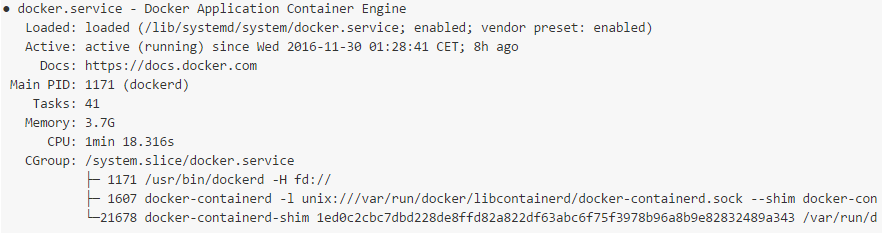
\includegraphics[width=1\columnwidth]{img/docker-services} 
\caption[docker services]{Services Docker opperationnel}
\label{fig:dockerservices} 
\end{figure}

Il faut à présent configurer Docker pour votre utilisateur hôte.

\begin{figure}[H] 
\centering
\begin{lstlisting}[frame=single]
$ sudo usermod -aG docker $(whoami)
\end{lstlisting}
\caption[Code - Configurer utlisateur Docker]{Configurer utlisateur Docker}
\label{fig:configUserDocker} 
\end{figure}

À se point ci, il vous faut redémarrer votre machine.

\subsubsection{Installation Docker-compose (1.9)}

\begin{figure}[H] 
\centering 
\begin{lstlisting}[frame=single]
$ curl -L "https://github.com/docker/compose/releases/download/1.9.0/docker-compose-$(uname -s)-$(uname -m)" -o /usr/local/bin/docker-compose
$ sudo chmod +x /usr/local/bin/docker-compose
$ docker-compose --version
\end{lstlisting}
\caption[Code - Installation Docker-compose]{Installation Docker-compose}
\label{fig:installCompose} 
\end{figure}

Vous devriez à présent obtenir la sortie console suivante:

\begin{figure}[H] 
\centering 
\begin{lstlisting}[frame=single]
docker-compose version: 1.9.0
\end{lstlisting}
\caption[Code - Docker-compose version]{Docker-compose version}
\label{fig:composeVersion} 
\end{figure}

\subsection{Téléchargements}

\section{Fonctionnement}
\subsection{Docker}
Il faut commencer par clarifier de quoi on parle lorsque l'on utilise le mot conteneur. Il s'agit d'une \emph{enveloppe} virtuelle permettant de packager une application ou un code avec toutes les dépendances nécessaires au fonctionnement de l'application. On package donc les fichiers source, librairies, runtime, outils, fichiers, base de données, etc. 

Un conteneur n'embarque pas de \gls{os}, il s'appuie sur celui de l'hôte sur lequel il est déployé. Ce qui rend un conteneur beaucoup moins lourd qu'une machine virtuelle \ref{fig:vs}.

Il faut également spécifier que Docker opère une isolation, des conteneurs, au niveau du système d'exploitation. 

Un conteneur Docker est décrit à l'aide d'un simple fichier \emph{.Dockerfile}, il décrit la création du conteneur, en détail. On peut personnaliser cette description de manière très détaillée. 

Il faut voir une application réalisée avec Docker comme une somme de microservices. Nous verrons dans la section suivante des exemples basiques d'application Docker. Le but étant de:

\begin{itemize}
\item rendre l'application davantage élastique;
\item améliorer les performances;
\item le déploiement continu est facilité. On peut relancer les services indépendamment les uns des autres.
\end{itemize}


\subsection{Docker-compose}
Docker-compose permet de définir et d'exécuter des applications multi-conteneurs. En effet, sans compose il fallait lancer les différents services de votre application soit manuellement soit en utilisant des scripts.

Compose utilise un fichier de composition, \emph{docker-compose.yml}, afin de configurer une application Docker. Ce qui permet de lancer une application à l'aide d'une seule commande. 

Pour résumer, une application Docker, utilisant Compose, est la combinaison de trois étapes:

\begin{enumerate}
\item Définir les différents Dockerfile des vos micro services composant l'application;
\item Définir les services qui seront utilisés dans le composé, leurs relations et leurs configurations;
\item Lancer l'application avec la simple commande, \emph{docker-compose up}.
\end{enumerate}

\section{Exemples}
\subsection{simple pull, build et run}
Les trois commandes les plus importantes de Docker sont \emph{pull}, \emph{build} et \emph{run}. En effet, ces commandes sont indispensables et doivent impérativement être comprises.

Premièrement, intéressons-nous à la commande \emph{pull}:

\begin{figure}[H] 
\centering 
\begin{lstlisting}[frame=single]
$ docker pull debian:jessie

jessie: Pulling from library/debian
5040bd298390: Pull complete 
Digest: sha256:abbe80c8c87b7e1f652fe5e99ff1799cdf9e0878c7009035afe1bccac129cad8
Status: Downloaded newer image for debian:jessie
\end{lstlisting}
\caption[Code - Docker pull]{Docker pull}
\label{fig:dockerPull} 
\end{figure}

Avec cette commande l'engin Docker à téléchargé l'image de debian Jessie depuis le \emph{Docker Hub}. Vous pouvez trouver un grand nombre d'images sur \emph{Docker Hub} - \hyperref[Docker Hub]{https://hub.docker.com/}.

Il est possible de gérer les images contenues sur une machine hôte. La commande suivante permet d'afficher la liste des images:

\begin{figure}[H] 
\centering 
\begin{lstlisting}[frame=single]
$ docker images

REPOSITORY           TAG                 IMAGE ID            CREATED             SIZE
debian               jessie              e5599115b6a6        2 weeks ago         123 MB
\end{lstlisting}
\caption[Code - Docker images]{Docker images}
\label{fig:dockerImage} 
\end{figure}

Il est également possible de supprimer une image, afin de libérer de l'espace disque:

\begin{figure}[H] 
\centering 
\begin{lstlisting}[frame=single]
$ docker rmi e5599115b6a6

Untagged: debian:jessie
Untagged: debian@sha256:abbe80c8c87b7e1f652fe5e99ff1799cdf9e0878c7009035afe1bccac129cad8
Deleted: sha256:e5599115b6a67e08278d176b05a3defb30e5564f5be6d73264ec560b484514a2
Deleted: sha256:a2ae92ffcd29f7ededa0320f4a4fd709a723beae9a4e681696874932db7aee2c
\end{lstlisting}
\caption[Code - Docker rmi]{Docker rmi}
\label{fig:dockerRmi} 
\end{figure}

Je tiens a signaler que l'on peut déjà se rendre compte d'un avantage de Docker par rapport a une machine virtuelle, l'image de Debian que l'on vient de télécharger ne fait que 123MB.

À présent lançons notre premier conteneur Docker:

\begin{lstlisting}[frame=single]
$ docker run -it debian:jessie /bin/bash

root@47e35436f723:/# 
\end{lstlisting}


Il est maintenant possible d'exécuter n’importe quelle commande à l'intérieur du conteneur:

\begin{lstlisting}[frame=single]
$ date

Sun Feb  5 11:01:11 UTC 2017
\end{lstlisting}

\emph{Ctrl+d} permet de sortir du conteneur.

\begin{figure}[H] 
\centering 
\begin{lstlisting}[frame=single]
$ docker run -itd debian:jessie

5c09ebfa8bc99235ad482256dfb9fa1fa470a42314ed61654b6a653aff6fee6b
\end{lstlisting}
\caption[Docker run linux]{Docker run linux}
\label{fig:DockerRunLinux} 
\end{figure}

En ajoutant l'option "d" le conteneur est exécuté de manière \emph{détachée}.

En utilisant la commande suivant, il est possible de visualiser les conteneurs en cours d'exécution:

\begin{figure}[H] 
\centering 
\begin{lstlisting}[frame=single]
$ docker ps

CONTAINER ID        IMAGE               COMMAND             CREATED              STATUS              PORTS               NAMES
5c09ebfa8bc9        debian:jessie       "/bin/bash"         About a minute ago   Up About a minute                       admiring_brattain
\end{lstlisting}
\caption[Docker ps]{Docker ps}
\label{fig:dockerPs} 
\end{figure}

Il est possible d'exécuter n’importe quelle commande dans un conteneur en cours d'exécution:

\begin{figure}[H] 
\centering 
\begin{lstlisting}[frame=single]
$ docker exec -it admiring_brattain date

Sun Feb  5 11:06:21 UTC 2017
\end{lstlisting}
\caption[Docker exec]{Docker exec}
\label{fig:dockerExec} 
\end{figure}

Ici le conteneur est identifié par son nom, si à l'exécution aucun nom n'est défini, Docker en attribue un de manière aléatoire. Il est également possible d'identifier un conteneur en utilisant son \emph{CONTAINER ID}.

En effet, il est possible et bien utile de définir un nom à vos conteneurs:

\begin{figure}[H] 
\centering 
\begin{lstlisting}[frame=single]
$ docker run -itd --name inphinity debian:jessie

c4be3f837adcbd5ab077e2b4a7903d2c1d4b5c434c7f877079c3ab5e22a2c555

$ docker ps

CONTAINER ID        IMAGE               COMMAND             CREATED             STATUS              PORTS               NAMES
c4be3f837adc        debian:jessie       "/bin/bash"         3 seconds ago       Up 3 seconds                            inphinity
\end{lstlisting}
\caption[Docker run]{Docker run}
\label{fig:dockerRun} 
\end{figure}

Finalement, abordons la commande \emph{build}. En effet, pour le moment nous n'avons fait qu'utiliser des images déjà construites. Un aspect très intéressant de Docker est de pouvoir décrire en détail la construction d'une image qui sera ensuite utilisée afin de lancer notre conteneur.

Prenons comme exemple le cas ou vous souhaité lancer un conteneur qui possède Python 3 préinstallé dans la version que l'on souhaite.

Pour se faire, il faut créer un fichier \emph{Dockerfile} dans un dossier vide. Vous pouvez retrouver le fichier de cet exemple dans le dossier "sources" et en annexe.

\begin{enumerate}
\item Il faut spécifier l'image de base:
\begin{lstlisting}[frame=single]
FROM debian:jessie
\end{lstlisting}

\item On souhaite premièrement mettre à jour les paquets:
\begin{lstlisting}[frame=single]
RUN apt-get update && \
    apt-get upgrade -y
\end{lstlisting}

\item Finalement, on installe le paquet que l'on souhaite, python dans sa version 3:
\begin{lstlisting}[frame=single]
RUN apt-get install -y python3
\end{lstlisting}

\end{enumerate}

À présent, on peut \emph{build} notre image Docker, l'exécuter et voir que python 3 est bien présent:

\begin{figure}[H] 
\centering 
\begin{lstlisting}[frame=single]
docker build -t exemple_1 .

[...]
Successfully built dead33da7d24

$ docker run -it exemple_1

root@41ac57ce9c0f:/# python3
Python 3.4.2 (default, Oct  8 2014, 10:45:20) 
[GCC 4.9.1] on linux
Type "help", "copyright", "credits" or "license" for more information.
>>> 

\end{lstlisting}
\caption[Docker build]{Docker build}
\label{fig:dockerBuild} 
\end{figure}

\subsection{Serveur Web: Docker compose}
Afin de montrer l'utilisation de \emph{Docker Compose} nous allons réaliser un petit serveur web. Cela nous permettra également de voir comment plusieurs microservices encapsulés chacun dans un conteneur Docker, peuvent former une application.

Toutes les sources de cet exemple sont disponibles dans le dossier, \emph{$sources/exemple_2$}.

Cet exemple consiste en deux conteneurs Docker, construit à partir de deux \emph{Dockerfile}.

Premièrement, un conteneur avec mysql, qui gère la base de données:

\begin{figure}[H] 
\centering 
\begin{lstlisting}[frame=single]
FROM mysql:5.7

COPY ./my.cnf /etc/mysql/conf.d/
\end{lstlisting}
\caption[mysql Docker]{Msyql Docker}
\label{fig:mysqlDocker} 
\end{figure}

Deuxièmement, un conteneur avec PHP et apache, afin d'exécuter les pages web:

\begin{figure}[H] 
\centering 
\begin{lstlisting}[frame=single]
FROM php:7-apache

COPY php.ini /usr/local/etc/php/

RUN apt-get update \
  && apt-get install -y libfreetype6-dev libjpeg62-turbo-dev libpng12-dev libmcrypt-dev \
  && docker-php-ext-install pdo_mysql mysqli mbstring gd iconv mcrypt
\end{lstlisting}
\caption[php-apache Docker]{php-apache Docker}
\label{fig:phpApacheDocker} 
\end{figure}

De plus, les sources se trouvent dans se que l'on appelle un volumes, une source de données pour nos conteneurs. Dans cet exemple nous y mettons uniquement un fichier \emph{index.php} avec la commande \emph{phpinfo()}, afin de vérifier que notre application fonctionne bien.

Nous allons utiliser \emph{Docker Compose}, afin de lancer notre application complète:

\begin{figure}[H] 
\centering 
\begin{lstlisting}[frame=single]
$ nano docker-compose.yml

version: '2'
services:
  mysql:
    build: ./mysql
    environment:
      MYSQL_ROOT_PASSWORD: pass
    volumes:
      - db:/var/lib/mysql
  php:
    build: ./php
    ports:
      - '8080:80'
    volumes:
      - ./html:/var/www/html
    depends_on:
      - mysql
volumes:
  db:

\end{lstlisting}
\caption[Code - docker-compose configuration]{docker-compose configuration}
\label{fig:composeConfig} 
\end{figure}

Exécutons, à présent, notre application web:

\begin{figure}[H] 
\centering 
\begin{lstlisting}[frame=single]
$ cd exemple_2/
$ docker-compose up -d

[...]

Creating exemple2_mysql_1
Creating exemple2_php_1

$ docker ps

CONTAINER ID        IMAGE               COMMAND                  CREATED             STATUS              PORTS                  NAMES
e921dc5930ac        exemple2_php        "docker-php-entrypoin"   4 minutes ago       Up 4 minutes        0.0.0.0:8080->80/tcp   exemple2_php_1
cdb19eaa3cb7        exemple2_mysql      "docker-entrypoint.sh"   4 minutes ago       Up 4 minutes        3306/tcp               exemple2_mysql_1

\end{lstlisting}
\caption[Docker-compose up]{Docker-compose up}
\label{fig:composeUp} 
\end{figure}

Pour vérifier que tous fonctionnent, utilisez votre navigateur favori et accédez à l'adresse \emph{localhost:8080} \ref{fig:phpinfo}.

\begin{figure}[H] 
\centering 
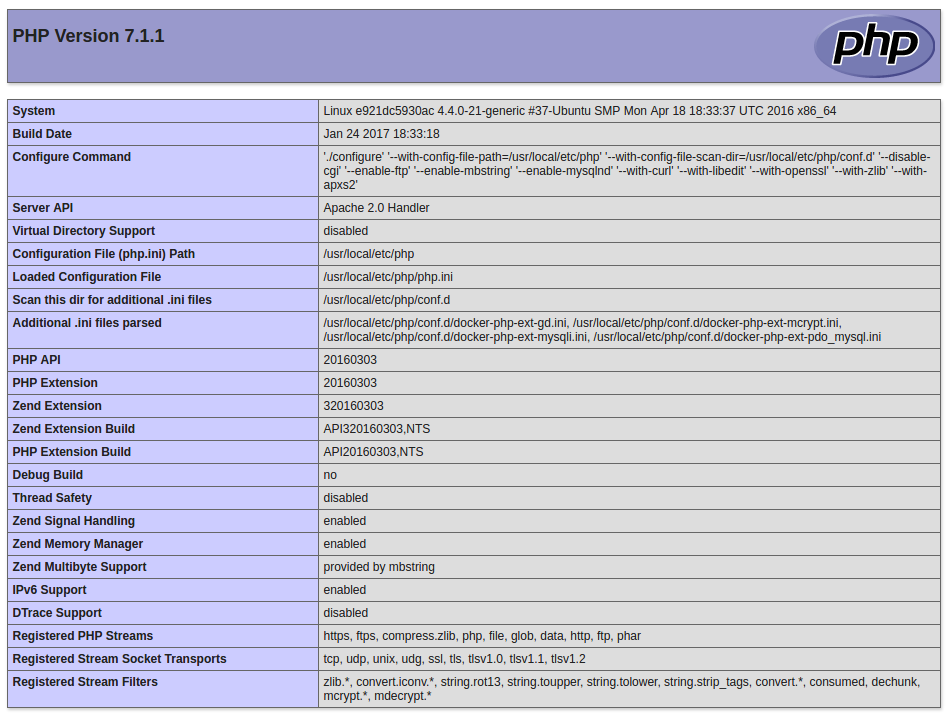
\includegraphics[width=1\columnwidth]{img/phpinfo} 
\caption[phpinfo]{phpinfo()}
\label{fig:phpinfo} 
\end{figure}

\subsection{Parallélisation}

Il est possible de lancer plusieurs conteneurs avec la même image. Nous allons utiliser ceci dans la suite du développement afin de lancer plusieurs conteneurs pour l'analyse des séquences.

\begin{figure}[H] 
\centering 
\begin{lstlisting}[frame=single]
$ docker run -itd debian:jessie

kamyh@kamyh-linux-tower ~/projects/master/documents/sources/exemple_2 $ docker ps
CONTAINER ID        IMAGE               COMMAND             CREATED             STATUS              PORTS               NAMES
8901929d2bf0        debian:jessie       "/bin/bash"         2 seconds ago       Up 1 seconds                            determined_sinoussi
877d2cddce6d        debian:jessie       "/bin/bash"         3 seconds ago       Up 2 seconds                            boring_nobel
4ff340b9c797        debian:jessie       "/bin/bash"         4 seconds ago       Up 3 seconds                            loving_mccarthy
e9a8bda7688f        debian:jessie       "/bin/bash"         4 seconds ago       Up 3 seconds                            focused_dijkstra
2060301458d6        debian:jessie       "/bin/bash"         5 seconds ago       Up 5 seconds                            awesome_blackwell
\end{lstlisting}
\caption[Docker Hmmer]{Docker Hmmer}
\label{fig:dockerHmmer} 
\end{figure}

Ici nous avons cinq conteneurs debian lancé simultanément. Ceci peut être très utile, par exemple, dans le cas d'une application web, afin de partager la charge des connexions utilisateurs entre plusieurs conteneurs.

































\chapter{Parallelisation python3}
\label{ch:parallel}

\section{Code de base}
\section{Utilisation}

\chapter{Environnement et application}
\label{ch:app}

Nous allons aborder, dans ce chapitre, le nouvel environnement créé a l'aide de Docker et le nouveau code produit à partir de celui de la thèse \thLeite.

L'environnement est réalisé à l'aide de \emph{Docker Compose}, il est composer de trois images différentes. Le code, orienté objet sera executé dans ce nouvel environnement.



\section{Images Docker}
Tous les fichiers necessaire à la construction des images de notre environnement se trouve dans le dossier \emph{$developpement/dockers$}.

\subsection{Hmmer}
La première image est celle visant à remplacer l'utilisation de l'\gls{api} en ligne de HMMER. Il sagit d'encapsuler l'application HMMER afin de pouvoir l'utiliser pour traiter les séquences protéinique.

Les fichiers necessaire se trouvent dans le dossier \emph{$developpement/dockers/hmmer$}. Il sagit d'un image basées sur \emph{centos}, qui est un image de base Docker très legere.

Tout d'abord, le \emph{Dockerfile} de cette image, install le compilateur C++ \emph{gcc}. Puis, il recupere les sources de l'application HMMER et les compilent.

Pour davantage de detail veuillez consulter directement le fichier \emph{Dockerfile} de l'image.

\subsection{Database}
L'application necessite plusieurs base de données Mysql. L'image \emph{database}, dont les sources se trouve dans le dossier \emph{$developpement/dockers/database$}, remplis cette fonctionnalitée.

Pour des raison de simplicité, cette image est construite à partir de Debian Jessie, la différence entre Centos et Debian est négligeable du fait que nous ne lanceront qu'un seul conteneur de cette image.

Due à la fois à la phase de débug et pour de futurs debug, l'image est construite avec un certains nombres de paquets afin de facilité la vie du developpeur.

La mise en place d'une image \emph{Docker} avec un serveur mysql n'est, par experience, jamais une chose facile à réaliser. C'est pour cela que nous allons entré un peu plus dans les détail les différentes commande qui composent le fichier \emph{Dockerfile} de cette image. Il n'est pas forcément necessaire de lire ce sous-chapitre pour comprendre les aboutissant de cette thèse, mais il est necessaire que les informations qui suivent y figure.

Premièrement, afin de pouvoir accèder au conteneur lancé à partir de cette image, il faut faire en sorte que mysql écoute les connexions en entrée.

\lstset{language=bash}
\begin{lstlisting}[frame=single]
RUN sed -i -e"s/^bind-address\s*=\s*127.0.0.1/bind-address = 0.0.0.0/" /etc/mysql/my.cnf
\end{lstlisting}

Maintenant que notre conteneur peut reçevoir des connexions, on install \emph{mysql-server mysql-client libmysqlclient-dev} qui installent Mysql sur notre image.

On peut démarrer le service Mysql:

\begin{lstlisting}[frame=single]
RUN mysqld &
RUN service mysql start
\end{lstlisting}

On oublie pas d'exposer le port de connection que l'on souhaite. Ici le 3306 qui est le port par défault de Mysql.

\begin{lstlisting}[frame=single]
EXPOSE 3306
\end{lstlisting}

On modifie également quelques configuration Mysql, afin de pouvoir utiliser des fichiers \emph{.sql} de tailles plus grandes.

\begin{lstlisting}[frame=single]
RUN sed -ire 's/max_allowed_packet.*=.*/max_allowed_packet = 200M/g' /etc/mysql/my.cnf
RUN sed -ire 's/key_buffer_size.*=.*/key_buffer_size = 128M/g' /etc/mysql/my.cnf
\end{lstlisting}

On ajoute le fichier \emph{startup.sh} et ont fixe qu'au lancement du conteneur il soit executé.

\begin{lstlisting}[frame=single]
ADD ./startup.sh /opt/startup.sh

CMD ["/bin/bash", "/opt/startup.sh"]
\end{lstlisting}

Regardons se que l'on trouve dans le fichier \emph{startup.sh}:

\begin{lstlisting}[frame=single]

if [ ! -f /var/lib/mysql/ibdata1 ]; then

	mysql_install_db

	/usr/bin/mysqld_safe &
	sleep 10s

	echo "GRANT ALL ON *.* TO admin@'%' IDENTIFIED BY 'root' WITH GRANT OPTION; FLUSH PRIVILEGES" | mysql

	# For 1_F1 DetectDomains.py
	echo "CREATE DATABASE phage_bact" | mysql
	mysql phage_bact < /tmp/db/phagesVD.sql
	mysql phage_bact < /tmp/db/bacteriaVD.sql
	mysql phage_bact < /tmp/db/interactionsVD.sql
	mysql phage_bact < /tmp/db/neg_interactionsVD.sql
	mysql phage_bact < /tmp/db/protdom_create.sql
	mysql phage_bact < /tmp/db/progress_create.sql
	mysql phage_bact < /tmp/db/progress_interaction_create.sql

    # For 3_F1 countScoreInteraction.py
	mysql phage_bact < /tmp/db/score_interactions_create.sql

	echo "CREATE DATABASE domine" | mysql
    mysql domine < /tmp/db/domTGo.sql
    mysql domine < /tmp/db/domPfam.sql
    mysql domine < /tmp/db/domPgmap.sql
    mysql domine < /tmp/db/domTInteract.sql

    # For 4_F1 FreqQtdScores.py
	mysql phage_bact < /tmp/db/qtd_scores_create.sql

	killall mysqld
	sleep 10s
fi

/usr/bin/mysqld_safe
\end{lstlisting}

Dans se script, on commence par donner les privilèges Mysql à l'utilisateur admin. Ensuite ont mets en place les différentes base de données, \emph{$phage_bact, domine$}, dont l'application à besoins. On crée ces deux base de données et leurs tables.

Dans l'éventualité ou l'on souhaiterais ajouter une nouvelle base de donnée c'est ici qu'il faudra ajouter la command Mysql de création.

De plus si l'on souaite ajouter des table ou données à une de nos base de données, c'est également dans se fichier qu'il faudra le faire.

Comme vous pouvez le voir tous les fichier \emph{.sql} necessaire sont placé dans le dossier \emph{$developpement/dockers/database/data$}.


\subsection{Core}
%image for bio-info!
Due à la fois à la phase de débug et pour de futurs debug, l'image est construite avec un certains nombres de paquets afin de facilité la vie du developpeur.

C'est véritablemenmt cette images qui contient tous se qui est necessaire à l'execution de l'aspect bioinformatique de l'application. C'est également elle qui controlle l'application, étant donné que cest dans se conteneur que le code de l'application est executé.

Comme pour l'image \emph{database} ont install les paquets necessaire à utiliser Mysql, \emph{mysql-server, mysql-client, libmysqlclient-dev} et python.

On install pip3, le gestionnaire de paquets pip pour python3:

\begin{lstlisting}[frame=single]
RUN apt-get install -y python3-pip r-base
\end{lstlisting}

On install aussi un des paquets les plus important de cestte image.

\begin{lstlisting}[frame=single]
RUN pip3 install biopython
\end{lstlisting}

Afin d'acceder à la base de donnée depuis le code python il nous faut installer le paquet:

\begin{lstlisting}[frame=single]
RUN pip install mysql-connector
\end{lstlisting}

Finalement, on install Docker, car il nous faudra pouvoir communiquer avec l'engin Docker de l'hôte, afin d'executer des conteneur de l'image HMMER.

\begin{lstlisting}[frame=single]
RUN apt-get install -y curl
RUN curl -fsSL https://get.docker.com/ | sh
\end{lstlisting}


\section{Docker Compose}
Maintenant que nous avons toutes les images necessaire à notre environnement applicatif orienté bioinformatique, nous allonms voir comment les combiner à l'aide de \emph{Docker Compose}.

La figure \ref{fig:architecture} montre l'architecture qui est mise en place à l'aide de \emph{Docker}.

\begin{figure}[H] 
\centering 
\includegraphics[width=0.7\columnwidth]{img/architecture} 
\caption[architecture]{Virtual machine vs Docker}
\label{fig:architecture} 
\end{figure}



\section{<<Inphinity>>}
%TODO: change title

%python3 trad
%classes
%config
%logs

















\chapter{Mise en place (Docker)}
\label{ch:setup}

\section{Get de source}
\section{•}
\chapter{Simplification d'usage}

\lipsum[1-2]

\chapter{Résultats et Benchmarks}

\lipsum[1-2]

\chapter{Améliorations}

\lipsum[1-2]

\chapter{Conclusion}
\label{ch:conclusion}

Ce projet propose une solution qui prend le partit d'utiliser la platforme \emph{Docker}, qui offre beaucoup d'avantages. Nottament en terme de déploiement sur différente machine hôte (différent developpeur/utilisateurs). De plus, même si pour le moment l'application n'est que dans une optique de démonstration, le fait de développer en utilisant \emph{Docker} permet de passer tres rapidement en phase de production. Il faut également noté que \emph{Docker} est souvent utiliser pour faire du déploiment continue.

Le code, précédement (thèse \thLeite) développé sous forme de scripts qui necessitait de nombreuses entrées utilisateurs, est maintenant complétement automatique. De plus, l'application peut etres executé plusieurs fois, en fournissant autant de fichiers de configuration que l'on souhaite. Chacune de ces executions est succeptible de produire un \emph{dataset} spécifique. Mais une execution peut aussi executer que certaines phase du traitement (\thLeite).

Travailler sur un code déjà existant, est une expérience très interessante, même si cela présente également des désavantages. Un avantage important, est le fait d'avoir la liberté de se concentré sur certains aspect uniquement et de cette manière de les approfondire davantage. C'est ce qui à été fait durant se travail avec l'idée de parallélisation et l'utilisation de la platforme \emph{Docker}.



% TODO: Remove before deadline
\chapter{Tables, Figures and Other Features}
This chapter shows example of picture and also serves to populate the different lists: list of figures, list of tables, bibliography, and glossary.

\section{Tables}
This section contains examples of tables.

\begin{table}[H]
\centering
\begin{tabular}{ccc}
\toprule
name & weight & food \\ 
\midrule
mouse	& 10 g	& cheese \\
cat	& 1 kg	& mice \\
dog	& 10 kg	& cats \\
t-rex	& 10 Mg	& dogs \\
\bottomrule 
\end{tabular}
\caption[A floating table]{A floating table.}
\label{tab:esempio}
\end{table}

\section{Figures}
This section contains examples of figures.

\begin{figure}[H] 
\centering 
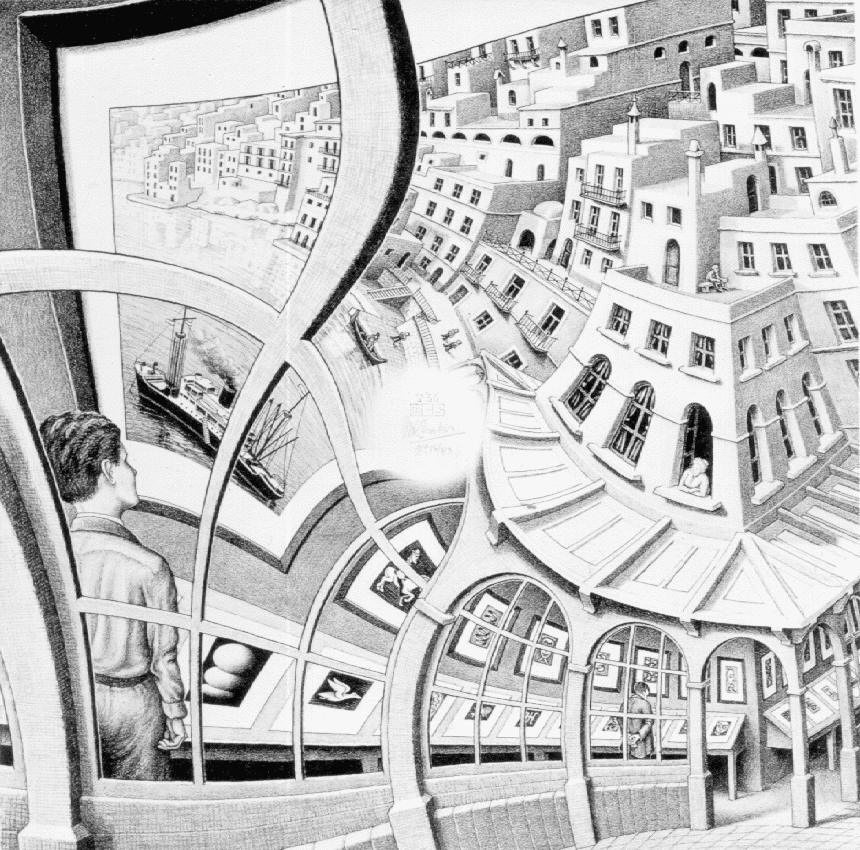
\includegraphics[width=0.5\columnwidth]{galleria_stampe} 
\caption[A floating figure]{A floating figure (the lithograph \emph{Galleria di stampe}, of M.~Escher, got from \url{http://www.mcescher.com/}).}
\label{fig:galleria} 
\end{figure}

\begin{figure}[H]
	\centering
	\begin{subfigure}[b]{0.45\textwidth}
		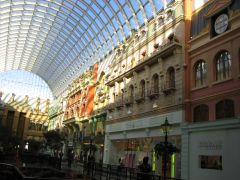
\includegraphics[width=\textwidth]{lorem}
		\caption{A gull}
		\label{fig:lorem}
	\end{subfigure}
	~ %add desired spacing between images, e. g. ~, \quad, \qquad, \hfill etc. 
	%(or a blank line to force the subfigure onto a new line)
	\begin{subfigure}[b]{0.45\textwidth}
		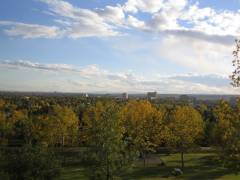
\includegraphics[width=\textwidth]{ipsum}
		\caption{A tiger}
		\label{fig:ipsum}
	\end{subfigure}
	~ %add desired spacing between images, e. g. ~, \quad, \qquad, \hfill etc. 
	%(or a blank line to force the subfigure onto a new line)
	\begin{subfigure}[b]{0.45\textwidth}
		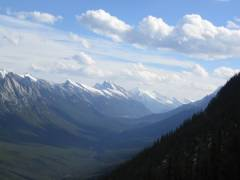
\includegraphics[width=\textwidth]{dolor}
		\caption{A mouse}
		\label{fig:dolor}
	\end{subfigure}
	~ %add desired spacing between images, e. g. ~, \quad, \qquad, \hfill etc. 
	%(or a blank line to force the subfigure onto a new line)
	\begin{subfigure}[b]{0.45\textwidth}
		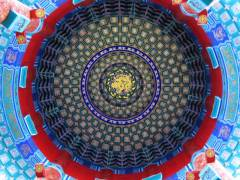
\includegraphics[width=\textwidth]{sit}
		\caption{A mouse}
		\label{fig:sit}
	\end{subfigure}
	\caption{Example subcaption}\label{fig:animals}
\end{figure}




\chapter{Another chapter}

\lipsum[3-12]


% Put your appendices here
\appendix
\chapter{Annexes}

\begin{itemize}
\item \thLeite -- <Thèse de Master 1108 VF.pdf>
\end{itemize}


% ----------------------------------------------------------------------------
% Backmatter
% ----------------------------------------------------------------------------
\backmatter

% Bibliography
\cleardoublepage
\begin{thebibliography}{99}
\bibitem{EinsteinPR1935}A.~Einstein et N.~Rosen, Phys. Rev.
\textbf{48}, 73 (1935)
\end{thebibliography}

% Glossary
\printglossaries
\end{document}

